\chapter{Introduction}
\label{chap1}

\section{Problem Statement}
\label{sec:problem-statement}

Remote controlled model aeroplanes have been in use for decades and have been a favourite among hobbyists for almost equally long. However, the past decade has arguably seen the greatest increase in computing power and efficiency since the silicon transistor was first invented (refer to the law popularised by~\citeauthor{moore2005cramming}, \citeyear{moore2005cramming}). Thanks to the growth in the mobile technology industries, computers have not only grown more powerful, but also smaller, lighter, cheaper and more power efficient. The increase in computing power and decrease in size and cost have made it possible to place small computers onto a model aeroplane with the aim of having it autonomously control, or semi-autonomously assist in controlling, a model aeroplane. 

Coupled with the rise in mobile computing power, control theory has also reached a point where it has a better understanding of the unstable, underactuated plant, such as a Segway, and manages to stabilise and control plants like these in some cases. One case of interest is a multirotor unmanned aerial vehicle (UAV) which resembles a model helicopter with multiple rotors. The so-called quadcopter configuration is of special interest for this research project.  

Autonomous UAVs are typically fitted with a multitude of sensors that provide the control system with the orientation and localisation data of the UAV.\@ These sensors normally include an accelerometer, gyroscope and GPS, along with others such as a barometer, optic flow sensor, magnetometer, etc. In its semi-autonomous state, the control system uses the sensor readings to keep the UAV level and stable while following a human pilot's flight instructions. Optionally, the pilot can engage the UAV in \emph{mission} mode where the UAV autonomously completes a flight mission selected by the pilot without the pilot controlling it. A mission consists of a set of GPS coordinate waypoints and altitudes for the UAV to follow. The pilot can also set the UAV to \emph{loitering} mode, where the UAV's control system will keep the UAV stable and level while holding the UAV's yaw angle and position constant. 

A consequence of the smaller and lighter sensors UAVs are typically e\-quipped with is that they are often less accurate than their larger, more powerful counterparts. The implication this holds for UAVs in general can readily be observed from most UAVs in \emph{loiter} mode where there is often significant drift around the UAV's set point. The accuracy of the individual sensors are often known or can be determined, but due to the mathematical filtering and fusion of the different sensor readings, as well as other operations that the control system may perform on the sensor data, it is difficult to determine the resulting accuracy of the position and orientation measurements made by the UAV's sensor suite. As a result, the pose (a vector describing an object's position and orientation) estimation accuracy of an outdoor UAV is not yet known. This research project attempts to find and implement an affordable and reliable method to determine the pose estimation error of a typical quadcopter UAV.\@  

\section{Project Motivation}

For many years, UAVs have mostly been the playthings of hobbyists and the researchers studying them. In recent years, however, the improvements that have been made to UAVs, which include quad-, hexa- and octocopters, and their controllers have drawn the attention of large corporations, such as Amazon and DHL, have expressed interest in incorporating UAVs into their respective workforces. 

Similarly, national governments have also noticed the increasing commercial and industrial potential that UAVs have, while also recognising the dangers that they pose to society if left unregulated. As such, many governments have moved to regulate and place restrictions on how and where UAVs may be used. The general trend of the regulations, as demonstrated by the regulations released by the~\cite{sacaa-drone-regs}, is that UAVs may be manually flown by a pilot anywhere below an altitude of $\SI{120}{\m}$, $\SI{50}{\m}$ away from people and buildings and $\SI{10}{\km}$ away from any aerodrome. These regulations allow for autonomous UAV flight, provided the UAV remain within radio line of sight of a human operator that can manually take over control of the UAV at any time should something go wrong. 

At the moment, UAVs are not as safe as they should be and can pose a serious health hazard to their surroundings and people if handled incorrectly. This, coupled with a general lack of hardware- and software-based collision avoidance capabilities, makes aviation authorities very cautious about allowing fully autonomous flight (i.e.\ out of radio line of sight). There are many safety improvements that can be made to UAVs, such as an improved control strategy, hardware improvements (such as rotor shrouds) and other fail-safe and collision avoidance systems. 

Having accurate pose data of a UAV in flight available is crucial to implementing an effective control strategy and collision avoidance system. As mentioned in Section~\ref{sec:problem-statement}, UAVs do not estimate their own pose very well and are prone to sensor drift over time. This allows for a `bubble' of pose uncertainty to be drawn around a UAV in flight, where the true pose of a UAV will be somewhere within the bubble, but the true pose is indeterminable. If the bubble's volume can be determined, it will allow a UAV's control system to generate safer, more efficient flight paths, which will improve the UAVs performance and make them a more attractive and safe option for governments and industry. Furthermore, the measurement system can be used to evaluate and improve the flight performance of a UAV.\@ 

\section{Potential Use Case}

The results from this research project will be applicable to many different industries and applications. To illustrate this, an example of where it would be helpful to know how accurately a quadcopter can estimate its pose is presented and briefly discussed. 

Concentrating solar power (CSP) is an attractive source of renewable energy which allows thermal energy to be stored for use at night time. However, a major hurdle to the construction of a CSP plant, in particular the central receiver configuration, is its hefty price tag. With CSP costing more per Watt than fossil fuels, as well as other renewable energy sources such as photovoltaic panels or wind turbines~\citep{irena-renewable_cost}, it is often difficult to convince financiers to invest in a central receiver CSP plant.

To prevent mirror deformation, wind loads, impacts from foreign objects and ground settling from affecting the heliostat's tracking path, each heliostat frame is designed to be heavy and sturdy and they are placed on strong foundations. They also come equipped with expensive actuators and gearboxes which minimise error build-ups during a heliostat's operation, contributing a significant portion to its total cost and~\cite{pitz2005ecostar} finds that approximately 40~\% of the initial capital expenditure of a CSP plant is spent on the thousands of heliostats placed around the receiver tower. 

CSP as a concept is old and well documented, but the technologies used are still relatively new and widely researched. As such, CSP plant design has not yet reached full maturity in terms of efficiency and optimal design. Therefore, there are still ways to reduce the cost of CSP plants, such as improving the heliostat control scheme, optimising heliostat design and improving the thermal storage mechanisms, amongst others~\citep{irena-cost_reduction}.  

Given the sheer size of a typical heliostat field, a small displacement in a mirror could influence the accuracy and effectiveness of that heliostat which is extremely undesirable given the lengthy calibration process required. Stellenbosch University (SU) and its Solar Thermal Energy Research Group (STERG) are attempting to make heliostats lighter, cheaper and reduce the need for expensive actuators and gearboxes, thereby allowing the heliostats to be placed on cheaper foundations with cheaper, less accurate actuators. This will lead to significant cost savings in a CSP plant's manufacturing stage. However, to achieve this without compromising the accuracy of the heliostats during operation, the lengthy calibration procedure currently in use may have to be optimised and possibly redesigned to allow the heliostats to be calibrated more often on a monthly, or even weekly, basis.

The current calibration procedure uses the sun as a light source and a section of the receiver tower as a reference target. This constrains the process to take place in day time and only allows one heliostat to be calibrated at a time. Since a heliostat field typically contains several thousand heliostats, this procedure may become very time-consuming. See Figure~\ref{fig:cur-calib-proc} for a diagrammatical example of the calibration procedure.

\begin{figure*}
  \centering
  \begin{subfigure}{0.49\textwidth}
    \centering
    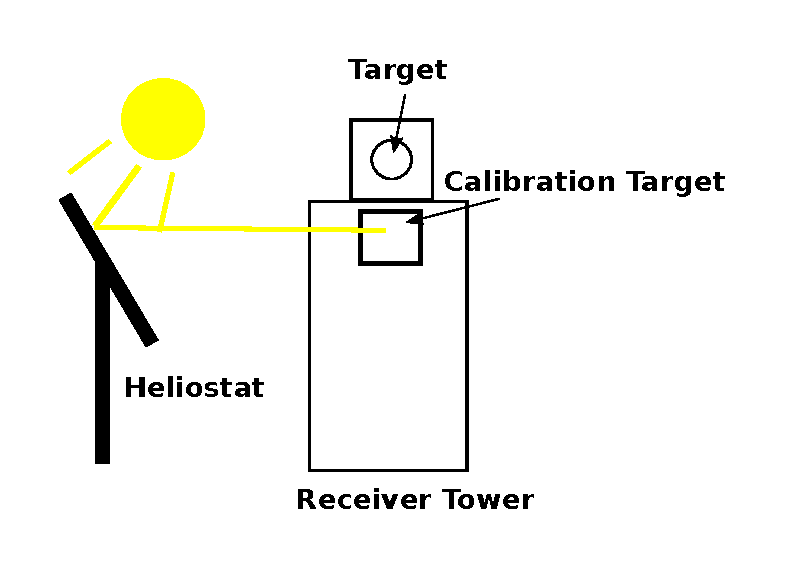
\includegraphics[width=\textwidth]{figures/chapter1/cur_proc.pdf}
    \caption{Diagram of the current heliostat calibration procedure where the position of the reflected sun rays on the target are measured.}
\label{fig:cur-calib-proc}
  \end{subfigure}%
~
  \begin{subfigure}{0.49\textwidth}
    \centering
    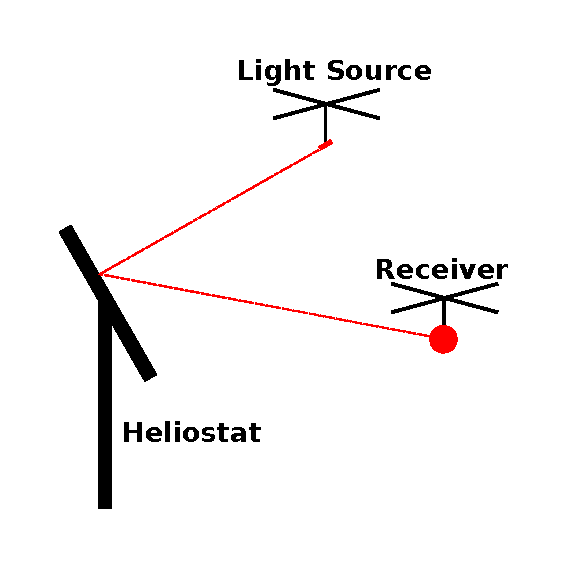
\includegraphics[width=0.72\textwidth]{figures/chapter1/drone_proc.pdf}
    \caption{A diagram of a proposed calibration procedure using quadcopters where the two quadcopter's positions are simultaneously measured.}
\label{fig:drone-calib-proc}
  \end{subfigure}
  \caption{A side-by-side comparison of how heliostats are currently calibrated and how heliostats can be calibrated by autonomous quadcopters.}
\label{fig:calib-diagrams}
\end{figure*}

In this regard, STERG is investigating the possibility of using quadcopter UAVs to autonomously perform or assist with heliostat calibration by, for example, making one quadcopter the light source and another the receiver. This will allow as many heliostats to be calibrated simultaneously as there are pairs of quadcopters available. See Figure~\ref{fig:drone-calib-proc} for an illustration of the proposed calibration procedure. Since the heliostats must be calibrated with a fine degree of accuracy, this approach requires an estimate of the quadcopter's pose estimation error. Here, the pose estimation error refers to the difference between a quadcopter's on-board pose estimate and its real pose.

Since a quadcopter typically drifts around its set-point, some pose error term must be included into the heliostat calibration procedure. First the expected pose error, or `bubble' of pose uncertainty, needs to be determined. After this is done, the pose error can be included into the calibration procedure and the procedure can be designed and refined around it.

Currently, the only pose measurements of a quadcopter available are its own on-board estimates produced by a combination of readings from its sensor suite, which typically includes a gyroscope, accelerometer and GPS.\@ However, the on-board data cannot be used here, since its error has not yet been quantified. Consequently, another approach is required to determine a quadcopter's pose estimation error. 

With a quadcopter's pose estimation error determined, it would be possible to autonomously calibrate a heliostat on a regular basis, which would lead to significant cost savings and allow CSP technology to become a more serious competitor in the renewable energy generation arena.



%The pose error of indoor quadcopters have been determined before with indoor motion tracking and measurement systems, such as the Vicon motion tracking system which has been shown to have millimetre-levels of accuracy~\cite{richards1999measurement}. However, these results and measurement methods are not applicable in the outdoor case, since testing indoors would deny a quadcopter its GPS coordinates. An outdoor quadcopter's GPS sensor readings provide an absolute position value, unlike its accelerometer, for example, whose readings are integrated twice to provide approximate position data, thereby making its readings prone to drift with time. Given the GPS sensor's importance to an outdoor quadcopter's localisation ability, it's crucial that a quadcopter have access to its GPS readings if we are to properly determine how well it estimates its pose, making it necessary to perform the measurements in the outdoors.  

\section{Existing and Proposed Solutions}

The current state-of-the-art method in determining the pose of a UAV in flight is to use an indoor motion tracking system, such as a Vicon\footnote{www.vicon.com/} system which uses a set of infrared cameras to track markers placed on an object. However, such systems cannot be used in this case since the UAVs of interest to this project require access to their GPS coordinates. The GPSs used in this project require a strong connection with a reasonably clear line of site to at least 6 different GPS satellites to produce accurate position data. These GPSs are also low-powered and small and therefore struggle to make good connections to satellites when indoors. Their line of sight to the satellites will also be affected, further reducing the GPS's accuracy. It was therefore decided that the quadcopters would be flown in the outdoors for this project. This implies that an outdoor pose measurement system is required. 

Outdoor pose measurement systems, such as radar- or laser-based systems, can also be used to perform pose measurements of a UAV.\@ However, these systems normally come at a premium cost. It was therefore decided to investigate and implement another pose measurement method that is cheap, accurate, repeatable and easy to use. 

The proposed outdoor UAV pose measurement system is based on computer vision techniques where the pose data of an object can be extracted from image or video data containing the object. The system consists of a camera to capture the image data and a computer to perform the pose data extraction. 

\section{Project Objectives}

The objectives of this research project are as follows. 

\begin{itemize}
  \item Design and implement a relatively cheap computer vision pose measurement system.
  \item Determine the measurement accuracy of the computer vision system.
  \item Use the computer vision system to determine the pose estimation accuracy of a demonstration quadcopter in flight. 
\end{itemize}

\section{Document Structure}

This document begins with a review of existing literature and of previous research results in the fields relevant to this project, such as computer vision techniques, UAV control strategies and others. Afterwards, the design and implementation, as well as the determination of the accuracy of the computer vision pose estimation system is discussed. This is followed by a discussion on how the pose measurement error of the computer vision system was determined for subsequent measurements and used to determine the pose estimation accuracy of a quadcopter in flight. Finally, a conclusion on the significant findings and results, as well as shortcomings and potential improvements, are presented. 
